% === INTRO === %

\vspace{1em}
\subsection{Una extensión del método de la potencia} \label{ap_A}

Vimos que una condición necesaria para la aplicación del método de la potencia es tener un autovalor dominante en módulo. ¿Qué sucede si esto no se cumple?

\vspace{1em}
\noindent Para simplificar el análisis separaremos en dos casos: 1. cuando hay autovalores dominantes iguales y 2. cuando no son iguales pero tienen el mismo valor absoluto.





% === 1 === %

\vspace{2em}
\subsubsection*{1. Método de la potencia para autovalores dominantes iguales} El método de la potencia se define por la siguiente relación de recurrencia:

\vspace{1em}
\begin{equation*} 
    b_{k+1} = \frac{\mathbf{A}b_k}{||\mathbf{A}b_k||} \qquad \forall k \in \mathbf{N}_0
\end{equation*}

\vspace{1em}
\noindent donde $b_0$ es un vector aleatorio, $||b_0||_2 = 1$.

\vspace{1em}
\noindent La demostración de convergencia de la serie definida por $\{b_k\}_{k \in \mathbb{N}_0}$ ---para $k$ par--- se basa en la siguiente igualdad: 

\begin{equation} \label{eq_potencia}
    b_k = \frac{\sum_{i=1}^{n} a_i \ \lambda_{i}^{k} \ x_i }{||\sum_{i=1}^{n} a_i \ \lambda_{i}^{k} \ x_i||_2}
\end{equation}

\vspace{1em}
\noindent donde $a_i := b_0^t\ x_i$, y $x_i$ es el autovector asociado al $i$-ésimo autovalor de $\mathbf{A}$ ---$\lambda_i$---, tal que $|\lambda_1| > |\lambda_2| \geq ... \geq |\lambda_n|$.

\vspace{2em}
\noindent Si suponemos, en cambio, que $\lambda_1 = ... = \lambda_r$, tal que $|\lambda_1| > |\lambda_{r + 1}|$, vemos que la ecuación (\ref{eq_potencia}.) se puede reescribir de la siguiente manera:

%\vspace{1em}
\begin{equation*} \label{eq_limite}
    b_k = \frac{\sum_{i=1}^{n} a_i \ \lambda_{i}^{k} \ x_i }{||\sum_{i=1}^{n} a_i \ \lambda_{i}^{k} \ x_i||_2} \cdot \frac{\lambda_1^k}{\lambda_1^k} 
        = \frac{\sum_{i=1}^{n} a_i \ (\frac{\lambda_{i}}{\lambda_{1}})^{k} \ x_i}{\frac{1}{\lambda_{1}^{k}}\ ||\sum_{i=1}^{n} a_i \ \lambda_{i}^{k} \ x_i||_2}
        \leq \frac{\sum_{i=1}^{r} a_i\ (\frac{\lambda_{i}}{\lambda_{1}})^{k}\ x_i + \sum_{i=r+1}^{n} a_i \ (\frac{\lambda_{i}}{\lambda_{1}})^{k} \ x_i }{(\frac{|\lambda_{1}|}{\lambda_{1}})^k ||\sum_{i=1}^{n} a_i \ x_i||_2}
\end{equation*}

\vspace{1em}
\noindent y tomando el límite, vemos que $\frac{\lambda_{i}}{\lambda_{1}} = 1\ $ si $\ i \leq r\ $ y $\ (\frac{\lambda_{i}}{\lambda_{1}})^{k} \longrightarrow 0 \ \ \forall i: r + 1\ ...\ n$. Tal que $b_k$ converge a:

%\vspace{1em}
\begin{equation*}
    \lim_{k \to \infty} b_k = \sum_{i=1}^{r} c_i\ x_i  
\end{equation*}

\vspace{1em}
\noindent donde $c_i := a_i \cdot (||\sum_{i=1}^{n} a_i \ x_i||_2)^{-1}$. 


\newpage
\noindent Como $x_1$ ... $x_r$ son autovectores de $\lambda_1$, vemos que para $c_1$ ... $c_r$ arbitrarios (con la condición que exista $c_i \neq 0$):

%\vspace{1em}
\begin{equation*}
    \mathbf{A} \ \sum_{i=1}^{r} c_i\ x_i = \sum_{i=1}^{r} c_i\ \lambda_1\ x_i = \lambda_1 \sum_{i=1}^{r} c_i\ x_i
\end{equation*}

\vspace{1em}
En consecuencia, sin importar quienes sean los $c_i$, se cumple que $\sum_{i=1}^{r} c_i\ x_i$ es un autovector y $\lambda_1$ es su autovalor. Esto nos permite inferir que $\lambda_1 = ... =\lambda_r$ esta asociado no solo a un autovector, sino a un subespacio de dimension $ \leq r$, ya que esta sumatoria define una combinación lineal de los $x_i$.   

\vspace{1em}
Por lo tanto, en el caso donde hay autovalores dominantes iguales, el método de la potencia converge correctamente. Este resultado lo comprobamos experimentalmente como se ve en el gráfico (\ref{fig:autovalor_repetido}.), donde se observa que el vector inicial tiende a un autovector a medida que aumenta la cantidad de iteraciones del algoritmo.

\vspace{1em}
\begin{figure}[!htbp]
    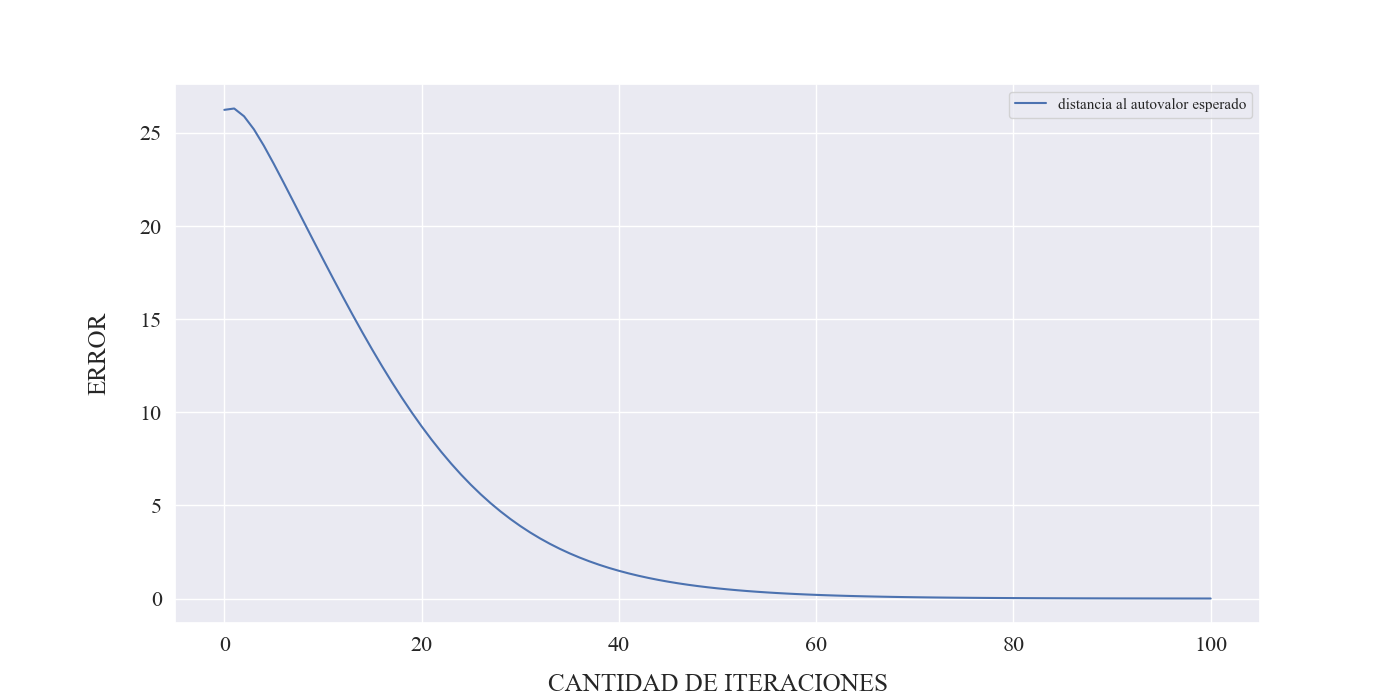
\includegraphics[scale=0.45]{files/src/.media/op_autovalor_repetido.png}
    \caption{Se eligió una matriz de $20 \times 20$ con base de autovectores y dos autovalores dominantes ($\lambda_1 = \lambda_2 = 20$). En cada iteración del método de la potencia medimos el error absoluto $||20 - \bar{\lambda}||_2$. Se puede observar como, a medida que aumenta la cantidad de iteraciones, la distancia entre el autovalor y el esperado tiende a cero.}
    \label{fig:autovalor_repetido}
\end{figure}

\vspace{1em}
Cabe destacar que, como $\sum_{i=1}^{r} c_i\ x_i$ es autovector para todo $c_i$ (tal que exista $c_i \neq 0$), entonces cualquier combinación lineal de los $x_i$ va a ser un autovector, y por ende hay infinitos resultados posibles con norma igual a uno ---a diferencia del caso en el que todos los autovalores son diferentes en módulo, donde hay solo dos autovectores con esta norma ---\footnote{Esto explica por qué hay que tener cuidado al comparar el autovector obtenido por el algoritmo con el que provee algún otro método, como $linalg.eig()$ de numpy.}.

\vspace{1em}
Algo interesante a notar es que, por tomar $k$ par, pudimos asumir que $signo(\lambda_1)^k = (\frac{|\lambda_{1}|}{\lambda_{1}})^k = 1$. Si no fueramos a asumir esto, observamos que en las iteraciones pares el método converge a $\sum_{i=1}^{r} c_i\ x_i$, pero en las impares, si $\lambda_1 < 0$, converge a $-\sum_{i=1}^{r} c_i\ x_i$. Ambos son autovectores válidos linealmente dependientes. Por lo que la restriccion de $k$ par no es necesaria para encontrar un autovector.

\vspace{1em}
Sin embargo, teniendo en cuenta que el método depende de la distancia entre una iteración y su consecutiva ---al comparar por tolerancia---, como en este caso el método oscila entre iteraciones pares e iteraciones impares, la distancia entre una iteración y su consecutiva no tenderá a cero. En consecuencia, de no imponer esta restricción, el método va a tener que hacer el total de las iteraciones $q$ sin poder interrumpirse antes. 




% === 2 === %

\vspace{2em}
\subsubsection*{2. Método de la potencia para autovalores diferentes pero iguales en módulo} 

Si suponemos, en cambio, que $|\lambda_1| = ... = |\lambda_r| > |\lambda_{r + 1}|$, vemos que $(\frac{\lambda_i}{\lambda_1})^k = signo(\lambda_i)^k\ \ \forall i: 1\ ...\ r$, y la ecuación (\ref{eq_potencia}.) se comporta de la siguiente manera:

\begin{equation*}
    \lim_{k \to \infty} b_k = \sum_{i=1}^{r} signo(\lambda_i)^k\ c_i\ x_i = \sum_{i=1}^{r} d_i\ x_i  
\end{equation*}

\vspace{1em}
\noindent donde $d_i = signo(\lambda_i)^k\ c_i$.

\vspace{1em}
\noindent Notamos que este vector oscilará si $k$ tiende al infinito irrestrictamente, ya que dependerá del signo de cada autovalor dominante. 

\vspace{1em}
Lo que es más, de tomar la subsecuencia convergente con $k$ par, $b_k$ no necesariamente será un autovector. Vemos que para $d_1\ ...\ d_r$ arbitrarios (con la condición que exista $d_i \neq 0$):

\begin{equation*}
    \mathbf{A} \sum_{i=1}^{r} d_i\ x_i = \sum_{i=1}^{r} \mathbf{A} d_i\ x_i = \sum_{i=1}^{r} \lambda_i\ d_i\ x_i 
\end{equation*}

\vspace{2em} 
\noindent Si existe al menos un $\lambda_j$ negativo, $1 \leq j \leq r$, entonces:

\begin{equation*}
    \sum_{i=1}^{r} \lambda_i\ d_i\ x_i = \lambda_1 \sum_{i = 1,\ i \neq j}^{r} d_i\ x_i - |\lambda_j|\ d_j\ x_j = \lambda_1 (\sum_{i = 1,\ i \neq j}^{r} d_i\ x_i - d_j\ x_j)
\end{equation*}

\vspace{1em} 
\noindent pero:

\begin{equation*}
    \sum_{i=1}^{r} d_i\ x_i \neq \sum_{i = 1,\ i \neq j}^{r} d_i\ x_i - d_j\ x_j
\end{equation*}

\vspace{1em}
\noindent por lo que el método de la potencia no converge a un autovector. 
Un ejemplo de esto se puede observar en el gráfico (\ref{fig:oscilante}.).

\vspace{1em}
Con este resultado en mente, observamos que en caso de computar la suma entre las últimas dos iteraciones del método de la potencia, para $k$ par lo suficientemente grande, obtendríamos lo siguiente:

\vspace{1em}
\begin{align*}
    b_k &= \sum_{i=1}^{r} c_i\ x_i \\
    b_{k+1} &= \sum_{i=1}^{r} d_i\ x_i = \sum_{i: \lambda_i > 0}^{r} c_i\ x_i - \sum_{i: \lambda_i < 0}^{r} c_i\ x_i \\ 
    b_k + b_{k+1} &= \sum_{i=1}^{r} c_i\ x_i + \sum_{i: \lambda_i > 0}^{r} c_i\ x_i - \sum_{i: \lambda_i < 0}^{r} c_i\ x_i   \\ 
    b_k + b_{k+1} &= 2 \sum_{i: \lambda_i > 0}^{r} c_i\ x_i
\end{align*}

\vspace{1em}
Es decir, estaríamos en la condición de la subsección anterior, por lo que este valor sí convergería al autovector asociado a $\lambda_1$.

\begin{figure}[!htbp]
    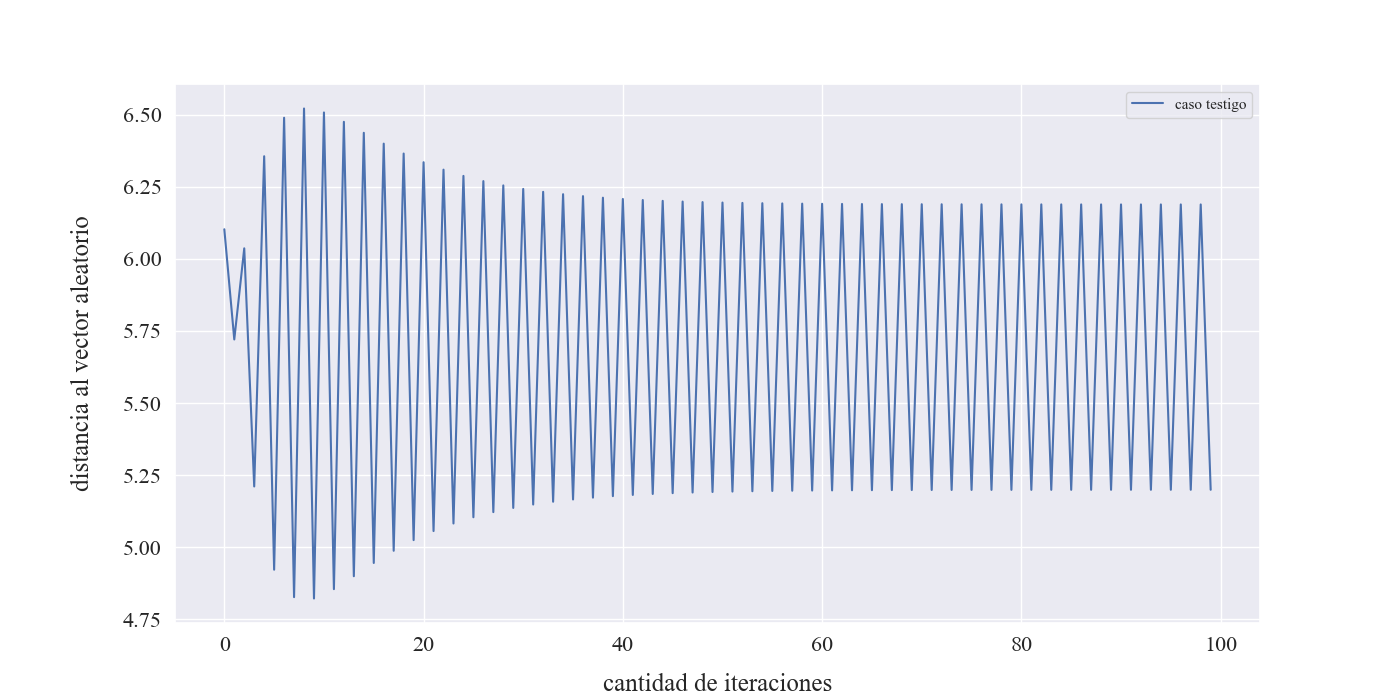
\includegraphics[scale=0.45]{files/src/.media/op_oscilante.png}
    \caption{Se eligió una matriz de $20 \times 20$ con base de autovectores y dos autovalores dominantes $\lambda_1 = 20$, $\lambda_2 = -20$. Además se seleccionó un vector aleatorio constante normalizado $v$. En cada iteración del método de la potencia calculamos la distancia $||v - y_k||_2$. Se puede apreciar como $v$ oscila entre las iteraciones pares e impares.}
    \label{fig:oscilante}
\end{figure}

\vspace{1em}

\vspace{1em}
Observamos que se podría calcular la resta para obtener otro autovector: el asociado a $\sum_{i: \lambda_i < 0}^{r} c_i\ x_i$. Es decir, podríamos obtener dos autovectores en un sólo llamado al método de la potencia. Como el método de la deflacíon asume que el método de la potencia encuentra de a un solo autovector por vez, decidimos no complejizar el algoritmo para aprovechar este caso puntual.




% === 3 === %

\vspace{2em}
\subsubsection*{3. El nuevo método} Con este resultado en mente planteamos el siguiente algoritmo como alternativa para el método de la potencia \textit{monte carlo}.

\vspace{1em}
\lstinputlisting[mathescape=true, escapechar=@, language=pseudo, label=potencia_modificada, caption={Pseudocódigo para una versión alternativa del \textit{método de la potencia}. El mismo soluciona el caso de autovalores en módulo repetidos.}]{files/src/.code/potencia_modificada.pseudo}

\vspace{1em}
Dada una matriz inicial cuyos autovalores pertenecen a los reales, este algoritmo permite calcular sus $k$ autovalores ---y vectores asociados--- no nulos. Esto permite relajar de manera considerable las restricciones del método original.
